\chapter{Implementación}

En este capítulo se revisará la implementación del diseño anteriormente descrito, con los resultados que se obtuvieron para cada etapa. El orden de la metodología descrita en el capítulo introductorio coincide con el orden en el que se implementó cada etapa, por lo que se aconseja tener presente la \hyperref[metodología]{metodología}.

La sección \textbf{Kinect} explica el proceso para realizar la instalación del software, calibración y pruebas de funcionamiento utilizando el sistema ROS en Linux. Se agrega una sección de problemas, en los que se identifica los mayores problemas encontrados en esta etapa.

Continuando con la sección \textbf{Hokuyo}, se procesede a mostrar el proceso de instalación del software, y se muestran algunas capturas que de nuevo demuestran el funcionamiento correcto de este sensor en ROS.

Posteriormente se realizan las pruebas de conexión entre un \textbf{STM32F4 y un roboclaw}, donde se realiza además el desarrollo de la librería de comunicación explicada en el capítulo de diseño.

La sección de \textbf{Encodificador de cuadratura} realiza un recuento del proceso de conexión entre el motor y el stm, además de la programación necesaria para realizar la lectura, y detalla algunos problemas encontrados para esta etapa.

La sección \textbf{Controlador PID} realiza un recuento de la implementación, sintonización y muestra los resultados de un cambio en la referencia a 0.5s.

El \textbf{Ensamblado de la base} se muestra en la sección correspondiente, donde además se proporcionan algunos videos de las primeras pruebas de funcionamiento del robot.

Finalmente, la sección \textbf{Protocolo de comunicación}, establece el proceso que se llevó a cabo para desarrollar esta librería, y muestra algunos de los problemas más importantes presentados durante el desarrollo de este proyecto.

El cálculo de la odometría, y la correción de problemas son secciones que llegan a culminar el proceso de diseño. Las secciones siguientes, denominadas \textbf{Implementación de gmapping y amcl}, realizan la implementación de los módulos necesarios para realizar la localización y navegación.

\newpage

\section{Kinect}
Lo primero a realizar, es instalar el entorno de ROS en una computadora con el fin de realizar pruebas con los módulos de ROS. Se realizó la instalación en un Chroot, dentro de una laptop personal corriendo ARCH Linux 4.17.10-1 utilizando la guía oficial de ROS Indigo que se puede encontrar \href{http://wiki.ros.org/ROS/Tutorials/InstallingIndigoInChroot}{aquí}.

El sistema resultante es una instalación de ROS Indigo dentro de un chroot de Ubuntu Trusty. El siguiente paso fué utilizar la librería de Iai Kinect \cite{iai_kinect2} para conectar un Kinect One (V2) a la computadora corriendo ROS. La figura \ref{F:kinect} muestra una imagen del Kinect que se utilizó durante las pruebas.

\begin{figure}[H]
\centering
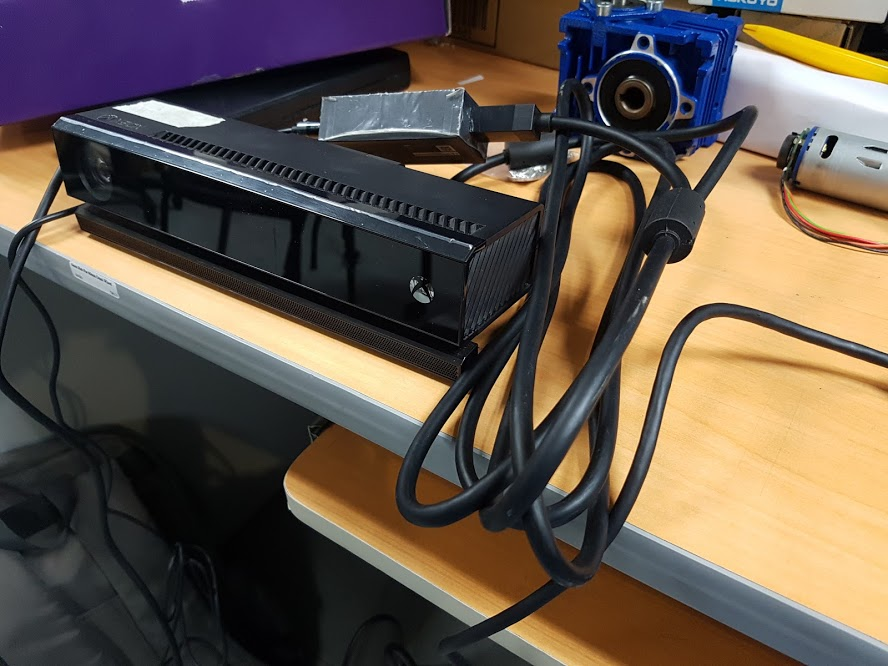
\includegraphics[scale=0.4]{imagenes/kinect.jpg}
\caption{Kinect One (V2) utilizado para realizar pruebas. Autoría propia.}
\label{F:kinect}
\end{figure}

\subsection{Instalación del software}

La instalación del software necesario se realizó siguiendo la guía del repositorio Iai Kinect 2, el cuál se puede encontrar \href{https://github.com/code-iai/iai_kinect2}{aquí}. La instalación depende del repositorio libfreenect2, el cuál se encuentra \href{https://github.com/OpenKinect/libfreenect2}{aquí}.

\subsection{Calibración del Kinect}

Siguiendo las instrucciones que se encuentran en el repositorio, lo primero a realizar cuando se instala el software adecuadamente, es proceder a generar los archivos de calibración para la cámara RGB e infraroja. Esto se logra realizando tomas a varios ángulos utilizando una imagen cuadriculada que proporciona el repositorio. Un ejemplo de esta imagen se muesntra en la figura \ref{F:cuadricula}.

\begin{figure}[H]
\centering
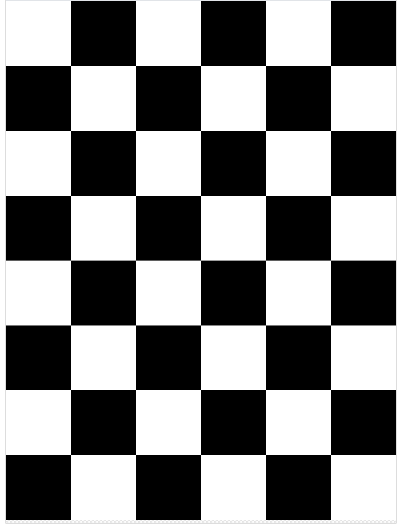
\includegraphics[scale=0.6]{imagenes/calibracion.png}
\caption{Imagen de calibración de prueba. Tomado de \cite{iai_kinect2}.}
\label{F:cuadricula}
\end{figure}

\subsection{Pruebas de funcionamiento}

A continucación, para lograr el funcionamiento correcto de la cámara, se debe correr roscore:

\begin{lstlisting}
roscore
\end{lstlisting}

Posteriormente, con la cámara conectada a la computadora, se procede a correr el nodo de ROS proporcionado por la librería Iai\_Kinect.

\begin{lstlisting}
roslaunch kinect2_bridge kinect2_bridge.launch
\end{lstlisting}

El resultado de este comando, se puede observar en la figura \ref{F:kinectsalida}.

\begin{figure}[h!]
\centering
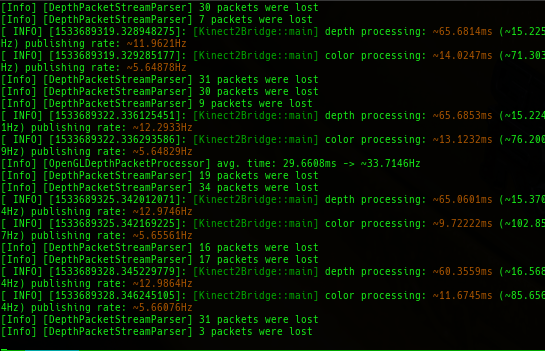
\includegraphics[scale=0.6]{imagenes/kinect_bridgesalida.png}
\caption{Resultado del comando kinect2\_bridge. Autoría propia.}
\label{F:kinectsalida}
\end{figure}

Una vez que este comando ha sido exitoso, se puede utilizar el siguiente comando para visualizar la salida:

\begin{lstlisting}
rosrun kinect2_viewer kinect2_viewer kinect2 sd cloud
\end{lstlisting}

Lo cuál produce la salida mostrada en las figura \ref{F:kinect1}.

\begin{figure}[H]
\centering
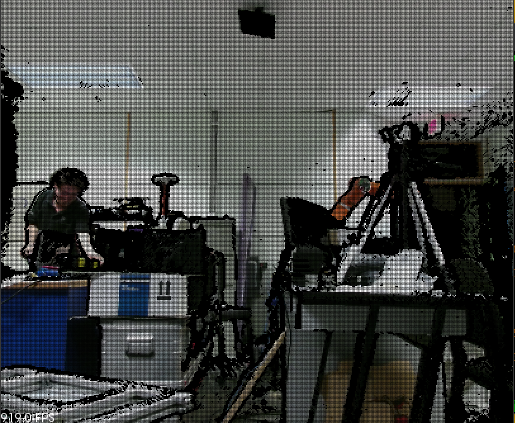
\includegraphics[scale=0.5]{imagenes/kinect_prueba.png}
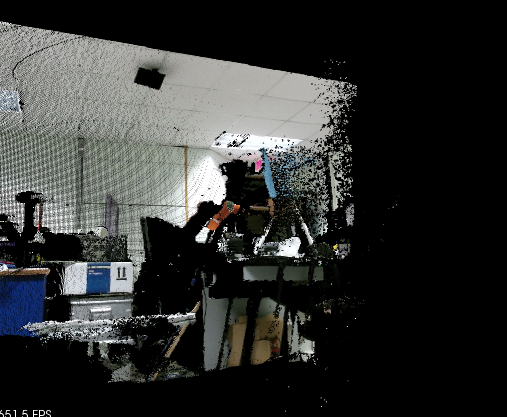
\includegraphics[scale=0.5]{imagenes/kinect_prueba2.png}
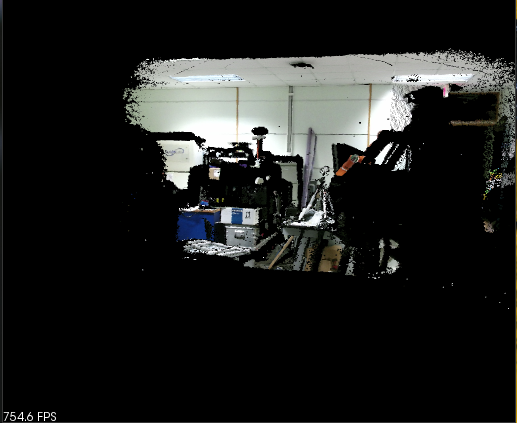
\includegraphics[scale=0.5]{imagenes/kinect_prueba3.png}
\caption{Prueba de la salida del kinect, utilizando el visor por defecto. Autoría propia.}
\label{F:kinect1}
\end{figure}

Finalmente, ROS posee una herramienta llamada \textit{RQT\_GRAPH}, la cuál ayuda a visualizar las conexiones entre los nodos y topicos siendo utilizados en el momento. Usando Rviz, y esta herramienta, vemos los topicos disponibles cuando se utiliza el nodo. La figura \ref{F:diagramakinect} muestra el resultado de \textit{RQT\_GRAPH}.

\begin{figure}[h!]
\centering
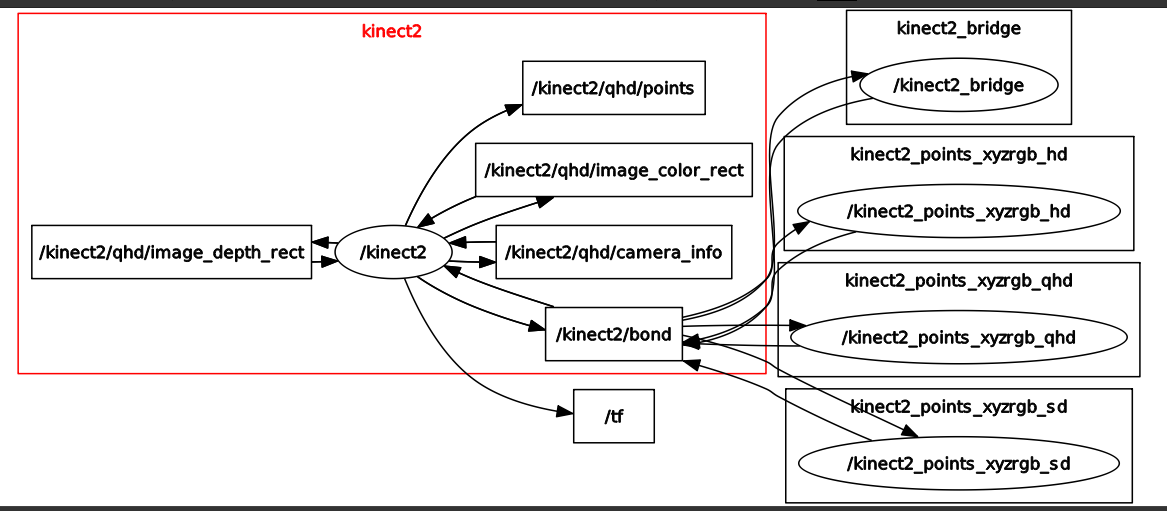
\includegraphics[scale=0.4]{imagenes/kinect_rqt_graph.png}
\caption{Esquema generado por RQT\_GRAPH que muestra las topicos disponibles por Iai Kinect. Autoría propia.}
\label{F:diagramakinect}
\end{figure}

\subsection{Problemas}

En esta etapa, el único problema que se encontró fué que el nodo de ROS por defecto no posee permisos para utilizar el USB, por lo que se le deben otorgar los mismos. La solución se menciona el repositorio libfreenect2.

\section{Hokuyo}

El uso del Hokuyo como parte del proyecto, es utilizar simplemente por razones de prueba. Se desea utilizar el Kinect en vez de este sensor pues es considerablemente más barato, y proporciona informacioón en 3D. Sin embargo, es posible que la navegación sea más sencilla utilizando un sensor 2D.

\subsection{Instalación del software}

La instalación es relativamente sencilla, pues consiste meramente en instalar un paquete de ROS llamando \textit{Hokuyo\_node}. La página oficial del paquete se encuentra \href{http://wiki.ros.org/hokuyo_node}{aquí}. Una vez instalado el paquete, iniciarlo es bastante sencillo.

\begin{lstlisting}
rosrun hokuyo_node hokuyo_node
\end{lstlisting}

\subsection{Pruebas de funcionamiento}

\begin{figure}[h!]
\centering
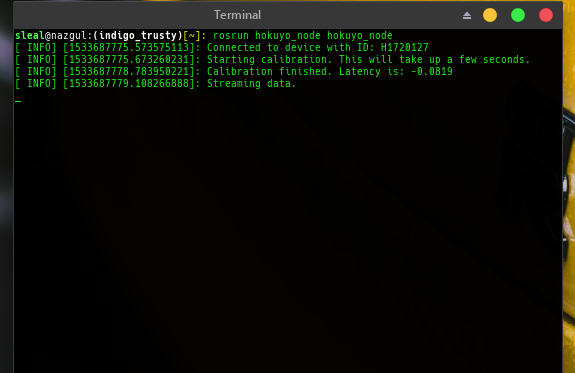
\includegraphics[scale=0.6]{imagenes/hokuyorosrun.png}
\caption{Inicialización correcta del módulo hokuyo\_node en ROS. Autoria propia.}
\label{F:hokuyonode}
\end{figure}

La figura \ref{F:hokuyonode} muestra la salida de la terminal que confirma que el módulo ha sido inicializado correctamente.

Utilizando \textit{RQT\_GRAPH} como se hizo anteriormente, se confirma que el nodo publica la información del laserscan correctamente en un nodo llamado \{\}scan, como era de esperarse. La figura \ref{F:hokuyorqtgraph} muestra la salida del programa.

\begin{figure}[h!]
\centering
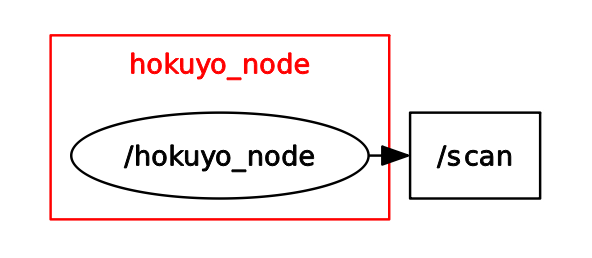
\includegraphics[scale=0.6]{imagenes/hokuyo_rqt_graph.png}
\caption{Diagrama generado por \textit{RQT\_GRAPH}, demostrando la salida de hokuyo\_node. Autoría propia.}
\label{F:hokuyorqtgraph}
\end{figure}

Además, la figura \ref{F:hokuyorviz} muestra la visualización del sensor laser, utilizando la herramienta \textit{Rviz}.

\begin{figure}[h!]
\centering
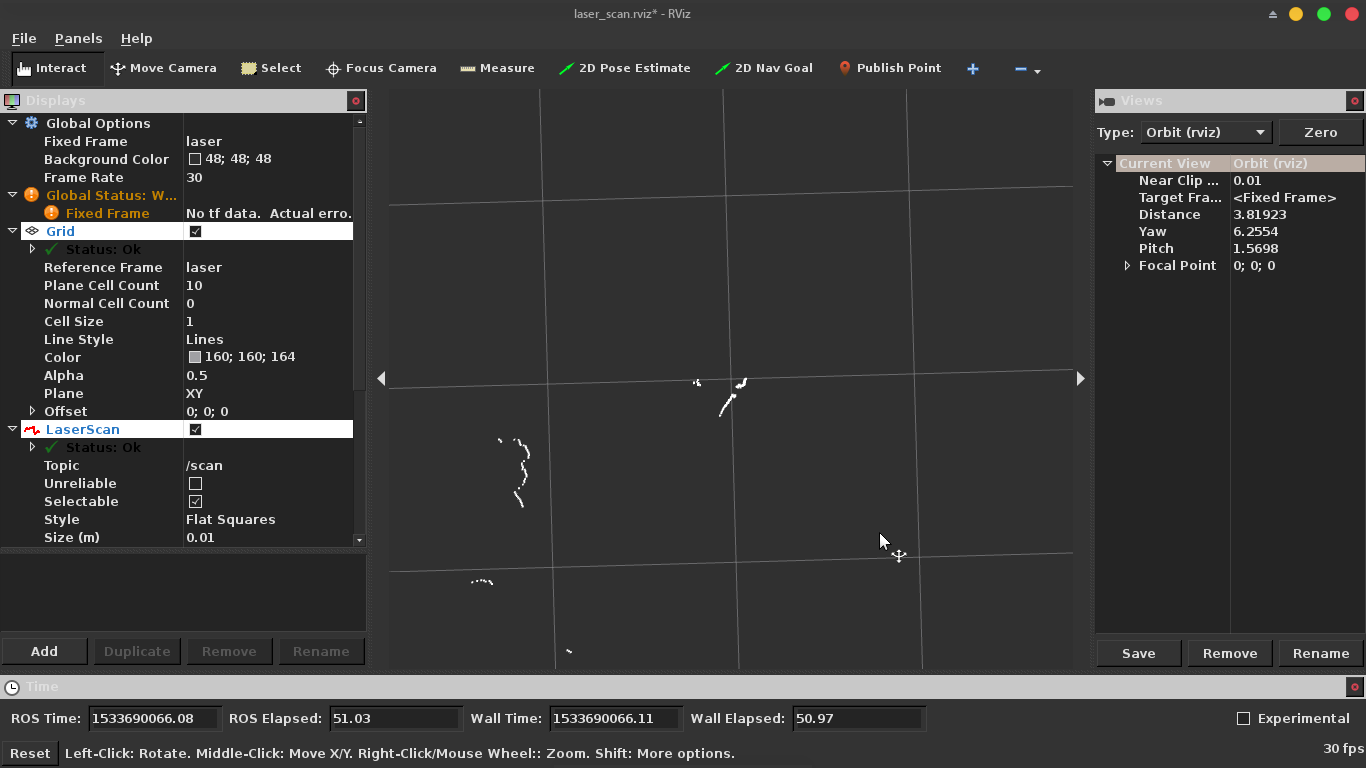
\includegraphics[scale=0.34]{imagenes/hokuyorviz.png}
\caption{Visualización de la salida del sensor láser Hokuyo utilizando Rviz. Autoría propia. }
\label{F:hokuyorviz}
\end{figure}

\subsection{Problemas}

Con las instalación del software \textit{Hokuyo\_node} no se encontró ningún problema.

\section{Conexión de un STM32F4 y un roboclaw}

Como se ha mencionado en capítulos anteriores, el STM32F4 será quién se conecta con la PC principal, recibe mensajes, y controla la velocidad de los motores enviando comandos de movimiento al Roboclaw. A continuación se muestra el proceso de conexión.

\subsection{Conexión}

Antes de iniciar con la conexión completa mostrada en la figura \ref{F:conexiones}, se realizaron pequeñas pruebas de comunicación, para diseñar la librería de comunicación, y probar la configuración correcta del equipo. La figura \ref{F:roboclaw-stm} muestra la conexión que se realizó.

\begin{figure}[h!]
\centering
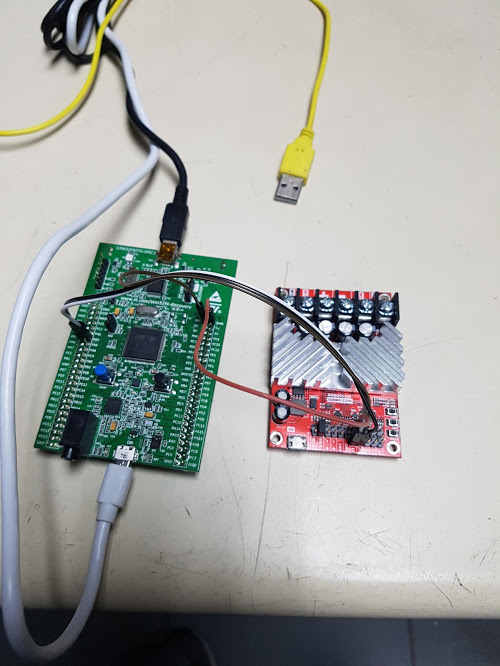
\includegraphics[scale=0.5]{imagenes/roboclaw-stm.jpg}
\caption{Conexión serial en los puertos USART de ambos dispositivos. Autoría propia.}
\label{F:roboclaw-stm}
\end{figure}

Para alimentar la parte lógica del controlador Roboclaw, existen dos opciones. Se puede configurar para alimentarse de la batería principal (de donde se toma energía para mover los motores) o se puede utilizar una alimentación lógica. Debido a que el STM32F4 no está diseñado para proporcionar suficiente corriente para una alimentación lógica de dos controladores, se optó por utilizar la opción de alimentación de la batería principal. La figura \ref{F:bateria} muestra la batería que se utilizó para realizar todas las pruebas.

\begin{figure}[h!]
\centering
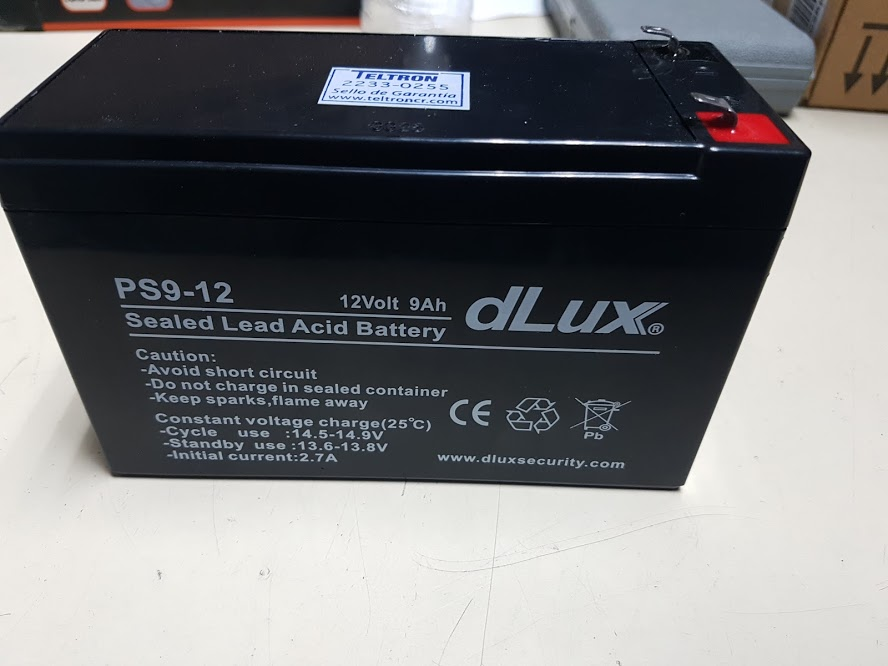
\includegraphics[scale=0.4]{imagenes/bateria.jpg}
\caption{Batería de 12V utilizada para alimentar a los controladores Roboclaw. Autoría propia.}
\label{F:bateria}
\end{figure}

El código que controla el microcontrolador stm32f411 se puede encontrar en el repositorio \href{https://github.com/arcoslab/stm32-roboclaw/}{stm32-roboclaw}. En específico el commit donde se realizan las primeras pruebas de conexión con el roboclaw se puede encontrar \href{https://github.com/arcoslab/stm32-roboclaw/commit/a6550243ac7c911bdcf5b3bf379690d89427ade5}{aquí}.

\subsection{Problemas}

En esta etapa del proyecto, las conexiones eléctricas eran bastante sencillas, pues realmente sólo se necesitan cuatro cables (RX, TX y dos tierras) para probar la conexión.

En el aspecto de la programación, fué fundamental la lectura del código escrito por IonMotion para realizar la misma tarea desde una computadora. El código mencionado se puede encontrar \href{http://www.basicmicro.com/downloads}{aquí}. El manual de Roboclaw también jugó un papel importante proporcionando la función que calcula el crc16 bits.

Posteriormente se realizaron cambios importantes a la librería, conforme algunos otros problemas fueron surgiendo. Por ejemplo se implementó una función ``padre'' que llamara a las instrucciones 0,1,4,5 según correspondiera.

Además, se reimplementaron las instrucciones de libopencm3 \textit{usart\_send\_blocking} y \textit{usart\_recv\_blocking} con timeout. El commit donde se realizó dicho cambio se puede encontrar \href{https://github.com/arcoslab/stm32-roboclaw/commit/de483b19c8b88b6c0c21cd51b446042f611a888b#diff-ceb3425682487491df75810266c27b6d}{aquí}.

\section{Encodificador de cuadratura}

\subsection{Conexión}

El sensor codificador de cuadratura, en el caso de los motores que se van a utilizar, utilizan un imán y dos sensores magnéticos con un desface mecánico de $45^\circ$ para producir las señales. La imagen \ref{F:encoderfisico} muestra el sensor mencionado.

\begin{figure}[h!]
\centering
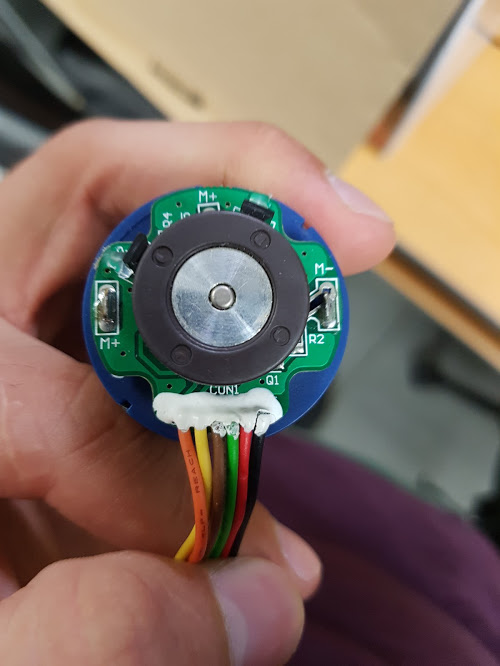
\includegraphics[scale=0.5]{imagenes/encoder.jpg}
\caption{Encodificador de cuadratura. Autoría propia.}
\label{F:encoderfisico}
\end{figure}

Del motor, salen 6 cables que se pueden observar en la figura \ref{F:cablesmotor}.

\begin{figure}[h!]
\centering
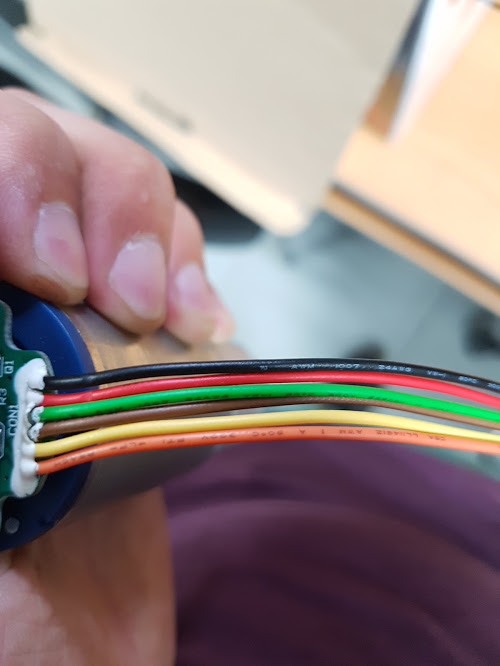
\includegraphics[scale=0.5]{imagenes/cables.jpg}
\caption{Cables del motor DC Actobotics. Autoría propia.}
\label{F:cablesmotor}
\end{figure}

Siguiendo el diagrama que se encuentra en la figura \ref{F:conexiones}, junto con el manual del fabricante de los motores, encontramos que la señal DC+ y DC- del motor son los cables rojo y negro respectivamente. La alimentación DC+ y DC- del sensor de cuadratura son los cables anaranjado y verde respectivamente. Finalmente el cable amarillo corresponde al canal A, mientras que el cable café corresponde al canal B. La figura \ref{F:actoboticscables} resume lo anteriormente descrito.

\begin{figure}[h!]
\centering
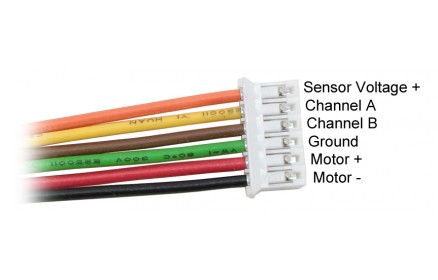
\includegraphics[scale=0.8]{imagenes/actoboticscables.jpg}
\caption{Cables de motor Actobotics. Tomado del manual de usuario.}
\label{F:actoboticscables}
\end{figure}

\subsection{Programación}

La programación de los cálculos del encoder de cuadratura conllevó varias iteraciones, puesto que hay varios factores a tomar en consideración. Por ejemplo, tomar en cuenta el caso en donde se da un rebase del contador del timer, y la acción a tomar una vez que esto sucede. La primera iteración funcional se puede ver en este \href{https://github.com/arcoslab/stm32-roboclaw/commit/c81a49b71de4a6a7cb5188abe2c16fd31c0b9cf0#diff-bff6209bf0949743f46f878a7d4c8c2c}{commit}. Sin embargo, si se observa la historia, la librería ha sufrido varios cambios posterior a estos.

Actualmente, existe un error con esta sección específica, por lo cuál debe ser revisada.

\subsection{Problemas}

Algunos de los problemas que se encontraron durante el desarrollo de esta sección son:

\begin{itemize}
\item En de las conexiones eléctricas debido a ``jumpers'' defectuosos.
\item En la PCB del sensor. Daño en los cables del motor, como se observa en la figura \ref{F:cables}.
\item Con la estructura del código, es específico la manera en la que se calcula la velocidad actual del motor.
\end{itemize}

\begin{figure}[h!]
\centering
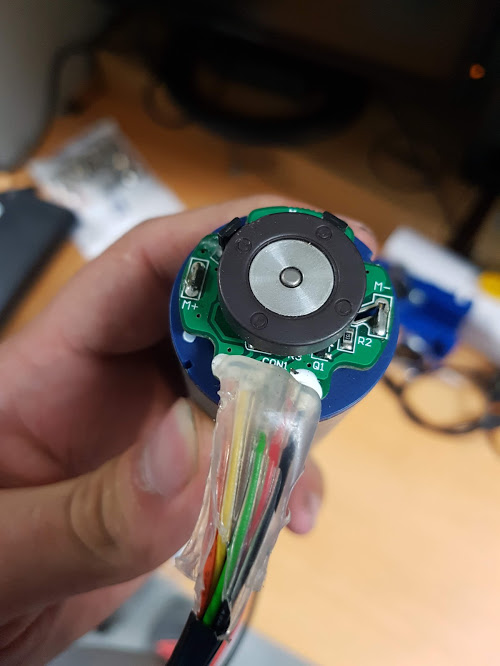
\includegraphics[scale=0.6]{imagenes/cablesmalos.jpg}
\caption{Reparación de cableado en un motor, debido a daños en las conexiones. Autoría propia. }
\label{F:cables}
\end{figure}

\newpage

\section{Controlador PID}

El controlador PID se diseñó con el propósito de ser una función completamente configurable. Por ejemplo, la frecuencia en la que se actualiza la velocidad actual, en ms es un parámetro, ya que se debe controlar la cantidad instrucciones que se mandan al roboclaw, para que las mismas no fallen. Además, los parámetros del límite superior, y las constantes de ganancia son configurables, como es de esperar.

\subsection{Impelementación}

La primera versión del código completo, junto con Kp, Ki, y Kd fué \href{https://github.com/arcoslab/stm32-roboclaw/commit/c8343d63d9700cd875b26012ce02b7371ca90b14#diff-33370e836e50db43bdb5933ccd61ab9e}{este} commit.


Anteriormente existieron otras iteraciones funcionales, pero únicamente tenían activados Kp y Ki.

\subsection{Sintonización}

La primera sintonización se realizó imprimiendo la informaicón en pantalla, y usando un algoritmo empírico propuesto por Federico Ruíz. Esta primera sintonización funcionó bastante bien para la mayoría de pruebas en el robot que se realizaron posteriormente. El algoritmo para sintonizar consiste en aumentar Kp hasta tener oscilaciones, regresar al punto donde no hay oscilaciones y aumentar Ki. Kd se utilizó en algunas pruebas, pero se determinó que no era necesario para la etapa en donde se encontraba el proyecto.

Es factible que posteriormente se haga un trabajo más profundo en lo que es la sintonización de este PID, sin embargo de momento no es un problema.

\subsection{Problemas}

\begin{itemize}
\item Algoritmo incorrecto de control PID
\item Fallo intermitente en las conexiones del encoder, lo cuál causaba errores difíciles de detectar
\item Cálculo incorrecto de las velocidades de cada motor, lo cuál afecta el control cerrado.
\item Mal ajuste de la frecuencia de comandos hacia el Roboclaw.
\end{itemize}

\subsection{Gráficas}

Debido a los últimos problemas inesperados en la odmetría del robot, se procedió a diseñar funciones de depuración en todos los aspectos anteriormente diseñados. Por lo tanto, se decidió realizar gráficas de la velocidad de los motores, y la posicón. Indirectamente estas gráficas muestran el funcionamiento del PID, donde se aplica un cambio en la referencia a los 0.5s. Las figuras \ref{F:pidposicion} y \ref{F:pidvelocidad} muestran lo anteriormente mencionado.

\begin{figure}[H]
\centering
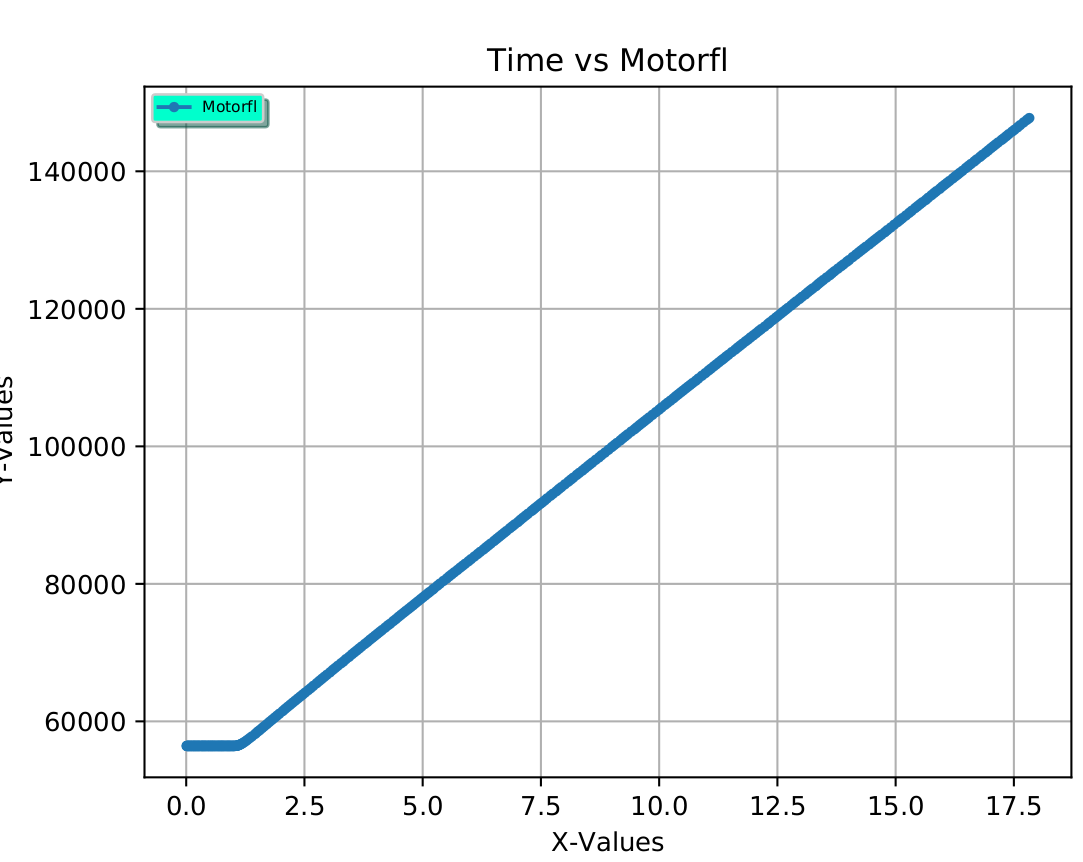
\includegraphics[scale=0.3]{imagenes/posicionpidmotorrr.png}
\caption{Tiempo versus la posición del motor en ticks del encoder, ante un cambio en la referencia en 0.5s. Autoría propia.}
\label{F:pidposicion}
\end{figure}

\begin{figure}[H]
\centering
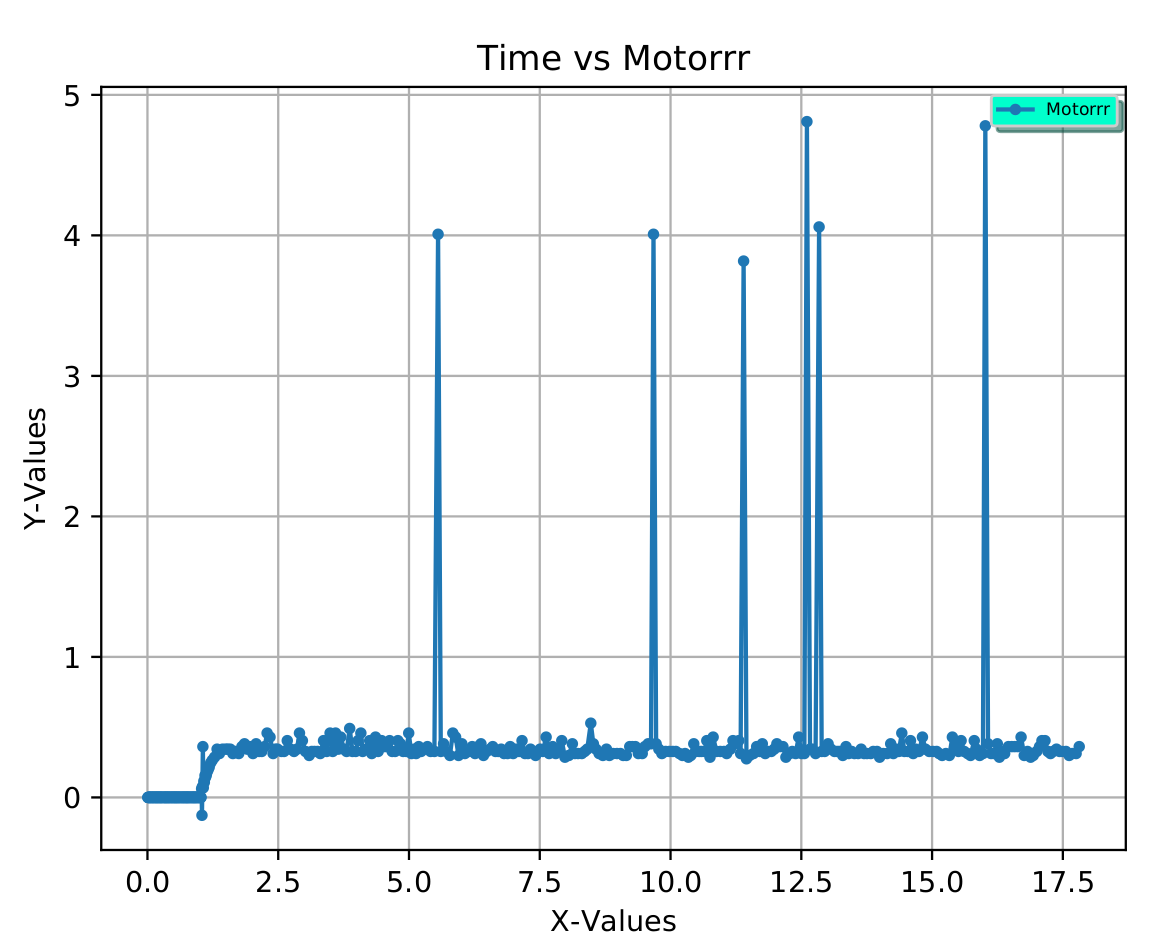
\includegraphics[scale=0.3]{imagenes/velocidadpidmotorrr.png}
\caption{Tiempo versus la velocidad del motor en rev/s, ante un cambio en la referencia en 0.5s. Autoría propia.}
\label{F:pidvelocidad}
\end{figure}

\newpage

\section{Ensamble de la base}

A continuación se muestran las capturas del ensamble. El proceso requirió armar ruedas junto con los acoples, y realizar todas las conexiones eléctricas. Las figuras \ref{F:ruedas}, \ref{F:ensamble1}, \ref{F:ensamble2}, \ref{F:ensamble3}, \ref{F:ensamble4} muestran el proceso de ensamblado.


\begin{figure}[H]
\centering
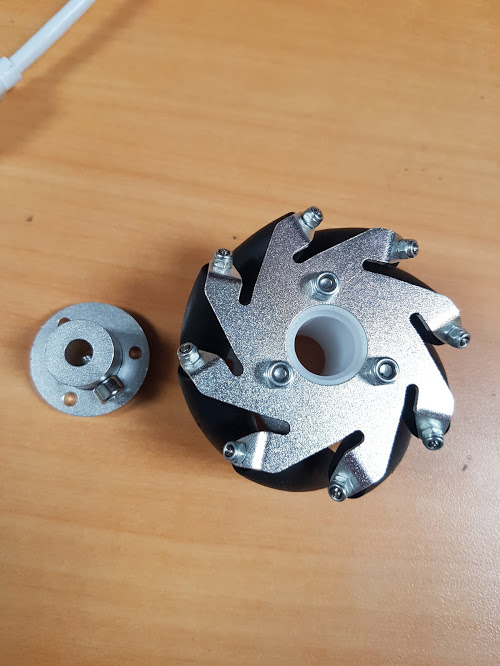
\includegraphics[scale=0.3]{imagenes/ruedas.jpg}
\caption{Acople y rueda a utilizar durante el ensamble. Autoría propia.}
\label{F:ruedas}
\end{figure}

\begin{figure}[H]
\centering4
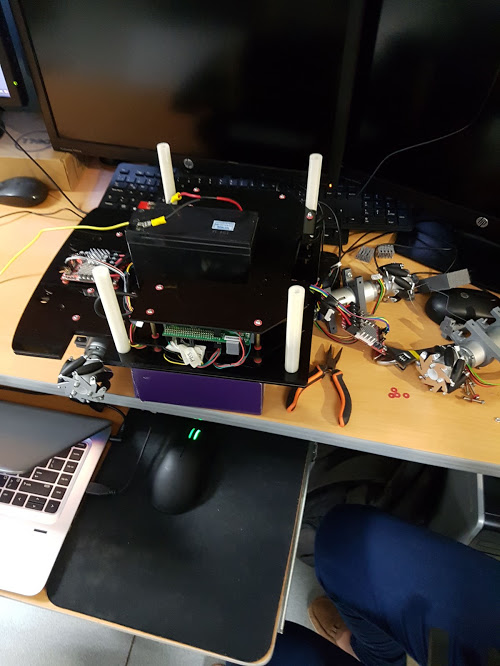
\includegraphics[scale=0.3]{imagenes/ensamble0.jpg}
\caption{Proceso incial del ensamble. Autoría propia.}
\label{F:ensamble1}
\end{figure}

\begin{figure}[H]
\centering
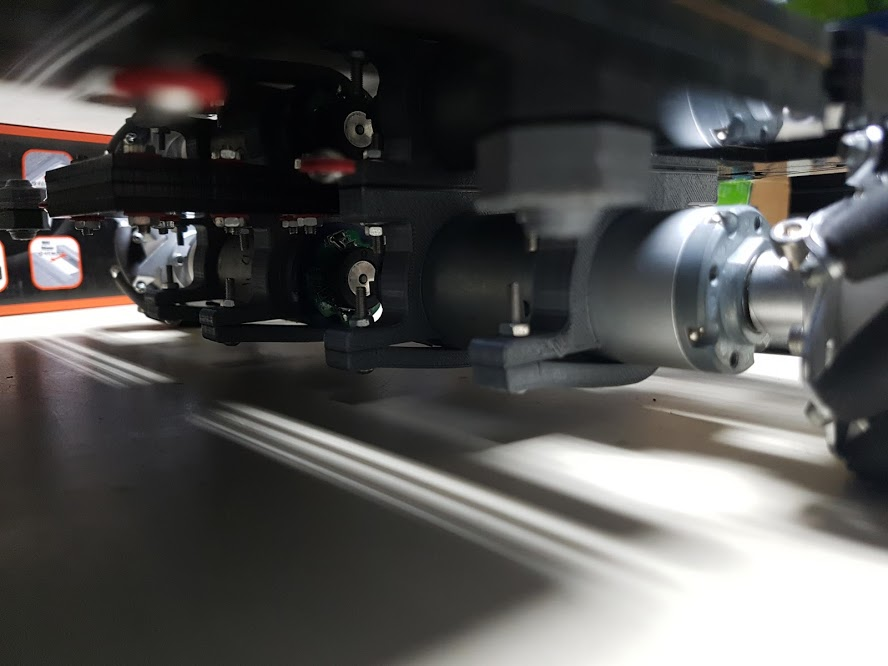
\includegraphics[scale=0.35]{imagenes/ensamble3.jpg}
\caption{Soporte de las ruedas. Autoría propia.}
\label{F:ensamble2}
\end{figure}

\begin{figure}[H]
\centering
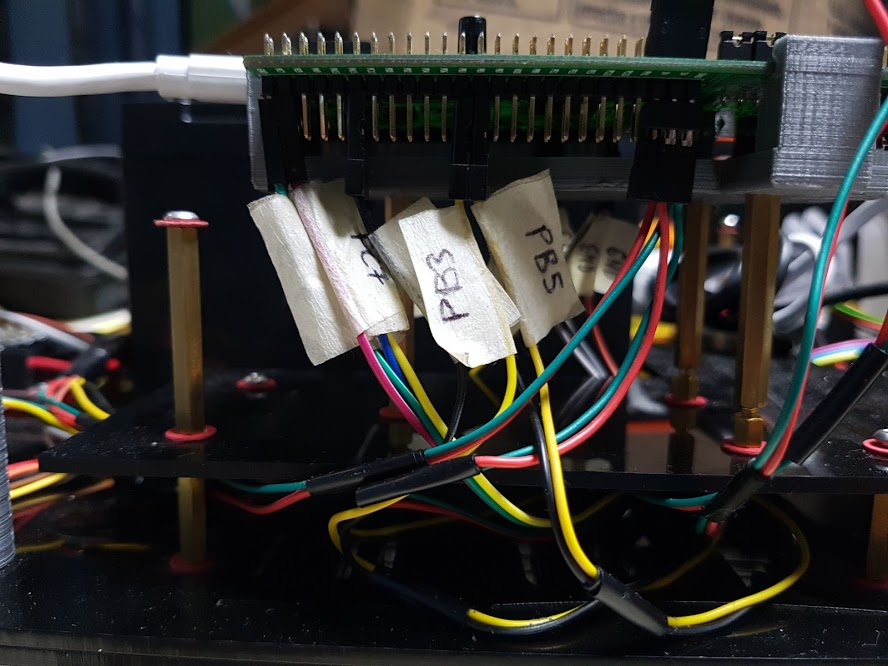
\includegraphics[scale=0.35]{imagenes/ensamble2.jpg}
\caption{Etiquetado de las conexiones. Autoría propia.}
\label{F:ensamble3}
\end{figure}

\begin{figure}[H]
\centering
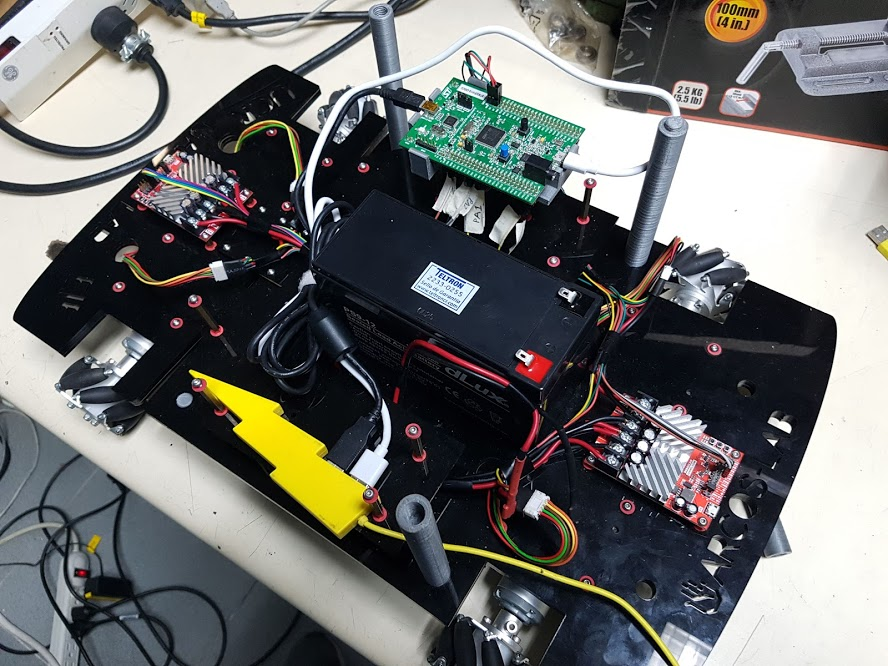
\includegraphics[scale=0.35]{imagenes/ensamble1.jpg}
\caption{Plataforma ensamblada totalmente. Autoría propia.}
\label{F:ensamble4}
\end{figure}

\subsection{Problemas}

\begin{itemize}
\item La mayor parte de los problemas relacionados con esta sección involucran el cableado eléctrico. Muchos de los cables utilizados no hicieron buen contacto, por lo que algunas conexiones no eran estables.
\item Falta de piezas impresas en 3D, y ruptura de algunas.
\end{itemize}

\subsection{Pruebas de movimiento}

A continuación en \href{https://photos.app.goo.gl/sycSZ52LNMN4YrVcA}{este} link se puede encontrar un video de la primera prueba de movimiento de los cuatro motores, junto con \href{https://photos.app.goo.gl/4x4wTcnVmySGP9ELA}{este} video, el cuál muestra los contadores de cada encoder incrementando durante la prueba.

\section{Protocolo de comunicación hacia la PC}

Para esta sección se realizaron varias iteraciones, y fué de los aspectos más problemáticos del proyecto.

\subsection{Prototipos y problemas}

Se inció con un protocolo que realizaba la transmición de información, enviando la información como un string, y no byte por byte. Es decir, 4.123 lo enviaría como 4 (1 byte), . (1 byte), 1 (1 byte), 2 (1 byte), 3 (1 byte). Esto hace que la transmición sea muy ineficiente, pues para un número flotante, que necesita 4 bytes para guardarse en memoria, se necesitan muchos bytes para mandarlo como string.

El mayor problema surgió dado que al ser variable la cantidad de datos que transmite (cuando se transmite 1.23 son cuatro byes, pero un número como 1.299999999999999 consume más bytes) es variable, se llenaba el espacio de memoria dinámica en la recepción, y el programa fallaba.

Por esta razón se implementó el segundo prototipo, el cuál manda toda la información en bytes. Esto provoca que la cantidad de datos transmitidos sean constantes, y el protocolo sea más eficiente. Además se agregó el checksum crc16 bits para no ejecutar instrucciones corruptas, pues esto en algún momento causó problemas también.

\subsection{Libopencm3-plus}

Existieron ciertos problemas con esta librería, puesto que una sección de código insertaba un ``\textbackslash r'' después de cada ``\textbackslash n'' en la transmisión serial. Este bug fué el problema más difícil de encontrar durante el desarrollo del proyecto.

\subsection{Problemas}

\begin{itemize}
\item Consumo de memoria dinámico por mal diseño de protocolo de comunicación.
\item Caractéres inesperados enviados por parte de la librería libopencm3-plus.
\end{itemize}

\section{Implementación del paquete en ROS}

El diseño del paquete en ROS se realizó utilizando como referencia código escrito para controlar el Robot llamado Neato. Esta librería se puede encontrar \href{https://github.com/mikeferguson/neato_robot}{aquí}. Nos interesa en particular, el código que se ecuentra dentro de neato\_robot/nodes/neato.py puesto que este script se encarga de subscribirse al tópico \textit{cmd\_vel} y publicar información de \textit{tf} y de \textit{odom}.

Se creó un repositorio con este código, el cuál se puede encontrar \href{https://github.com/slealq/omnidirectional_robot}{aquí}. En cuestión de problemas no se encontraron muchos, gracias a tener el ejemplo de código mencionado anteriomente. Se realizaron cambios de prueba en la frecuencia del nodo, sin embargo no hay cambios en la estructura como tal.

Las instrucciones de instalación del repositorio se encuentran en el \textit{README.md} del repositorio. La figura \ref{F:repositorio_installacion} muestra un ejemplo de las dependencias a instalar, y las instrucciones para instalar el paquete como tal.

\begin{figure}[H]
\centering
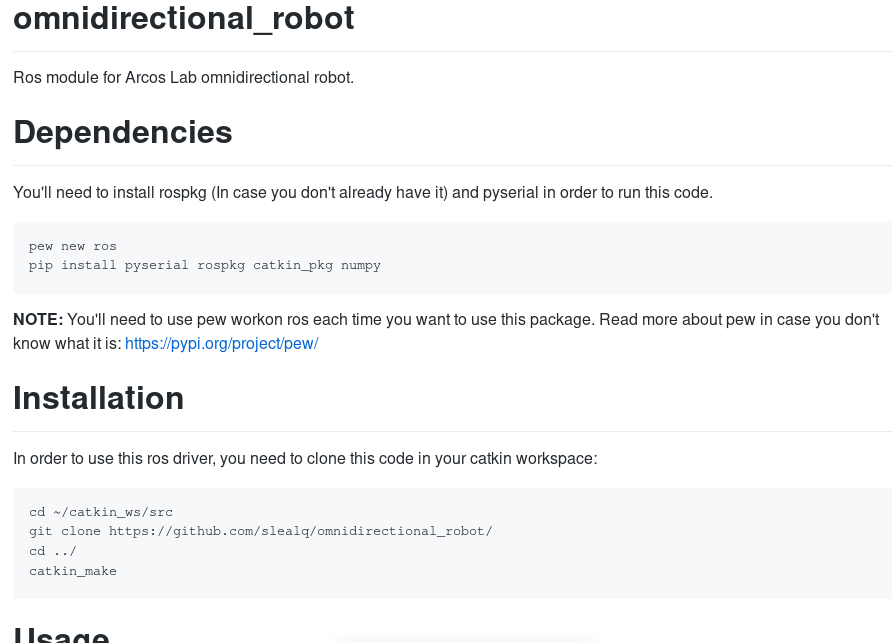
\includegraphics[scale=0.5]{imagenes/omnidireccional_instalacion.png}
\caption{Instrucciones de instalación e instalación de dependencias.  Autoría propia.}
\label{F:repositorio_installacion}
\end{figure}

El launch file que se debe correer para levantar el programa, es el que se encuentra en la dirección \textit{omnidirectional\_robot \textbackslash omnidirectional\_node \textbackslash launch \textbackslash bringup.launch}. Se levanta el nodo corriendo el siguiente comando, una vez que ya se tiene instalado el paquete con en Catkin correctamente.

\begin{lstlisting}
roslaunch omnidirectional_node bringup.launch
\end{lstlisting}

La visualización de los tópicos que se levantan cuando se corre este comando se puede observar en la figura \ref{F:rqtgraphomni}. En este punto, se encuentran levantados todos los tópicos necesarios para realizar la navegación.

\begin{figure}[H]
\centering
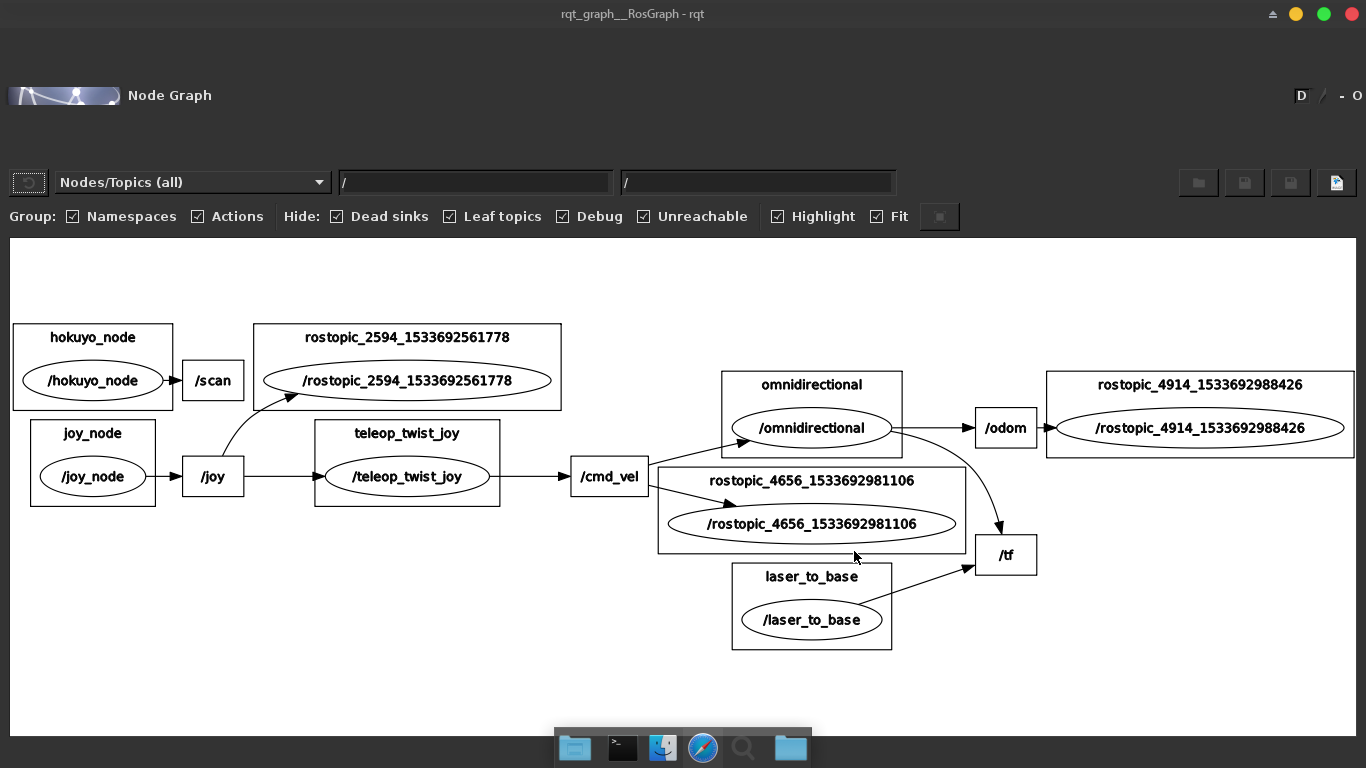
\includegraphics[scale=0.3]{imagenes/omnidirectional_rqtgraph.png}
\caption{Visualización de las relaciones entre tópicos y nodos levantas en ROS. Autoría propia.}
\label{F:rqtgraphomni}
\end{figure}

\section{Cálculo de la odometría}

El cálculo de la odometría se realizó hasta este punto, puesto que se necesitaba primero enviar comandos de movimiento hacia la base, y mover la base sobre alguna superficie para poder medir la veracidad de las mediciones de odometría.

\subsection{Problemas}

Las ecuaciones que se siguieron son realmente las mostradas en las sección de diseño, y no hubieron problemas en impelementar las ecuaciones.

Sin embargo, se encontraron varios problemas por resolver, algunos de los cuáles están relacionados a las interrupciones systick.

Cuando sucede una interrupción en Systick, se modifica el valor de las variables globales de posición. Si en un dado momento, el ciclo principal está realizando la transferencia de esta variable por comunicación serial, y el ciclo systick realiza una interrupción de hardware, el valor envíado por el puerto serial será incorrecto. Para esto se crearon unas variables temporales que se actualizan únicamente si una bandera de actualización se activa.

Por lo tanto, cuando se inicia una nueva comunicación serial, se desactiva una señal que deja de actualizar la variable de posición global, mientras se esté realizando la transmición de la variable. El diagrama mostrado en la figura \ref{F:main} se muestra este proceso, y la bandera \textit{update\_global\_pos} es la mencionada anteriormente.

\section{Pruebas y correción de problemas}

De las primeras pruebas que se realizó, fué verificar el movimiento correcto de la base omnidireccional utilizando el joystick. Se ajustaron los parámetros del PID de cada ruedas, para que el mismo fuera más rápido.

Realizando estas pruebas, fué donde se detectó el error mencionado del protocolo de comunicación, en donde la librería \textit{libopencm3-plus} tenía una pulga. Se detectó puesto que en momentos aleatorios del funcionamiento del carrito el stm32f411 quedaba en un estado de abort.

Utilizando gdb se obtuvieron pistas del problema, sin embargo no fué hasta leer el código contenido en la librería que se logró identificar el problema.

Posteriormente se realizó la verificación de la información obtenida de la odometría de las ruedas. Las pruebas que se realizaron fué medir con una cinta 1 metro, realizar marcas en el piso y realizar pruebas con movimientos hacia adelante, laterales y rotacionales.

El cuadro \ref{T:odometria} resume algunos resultados obtenidos de las pruebas.

\begin{table}[H]
\caption{Tabla de dos mediciones realizadas para comprobar el cálculo de odometría en la base. Autoría propia.}
\begin{tabular}{|l|l|l|l|}
\hline
Variable                 & Medición 1                                & Medición 2                                & Medición esperada (m)                     \\ \hline
X\_x                     & 1.034 m                                   & 1.045 m                                   & 1.000 m                                   \\ \hline
X\_y                     & 1.096 m                                   & 1.087 m                                   & 1.000 m                                   \\ \hline
$\alpha_z$ & $405^\circ$ & $395^\circ$ & $365^\circ$ \\ \hline
\end{tabular}
\label{T:odometria}
\end{table}

Como se puede observar, se muestran resultados bastante desviados de los valores reales. Esto se debe a errores o en el cálculo de la odometría, o en los parámetros de las ecuaciones de la kinemática.

Estos errores se deben corregir para poder implementar correctamente el algoritmo de SLAM.

\section{DualShock 4 en ROS}

Para conectar el control de PS4 a ROS, se utilizó un paquete llamado \href{https://github.com/solbach/ps4-ros}{ps4-ros}. Las instrucciones de instalación en el repositorio son bastante sencillas de seguir, por lo que esta etapa no demoró mucho. Una de las dependencias es utilizar un paquete llamado \href{http://wiki.ros.org/joy}{ros-joy} el cuál contiene la información del tipo de mensaje que se debe publicar para la información de un joystick.

\begin{figure}[H]
\centering
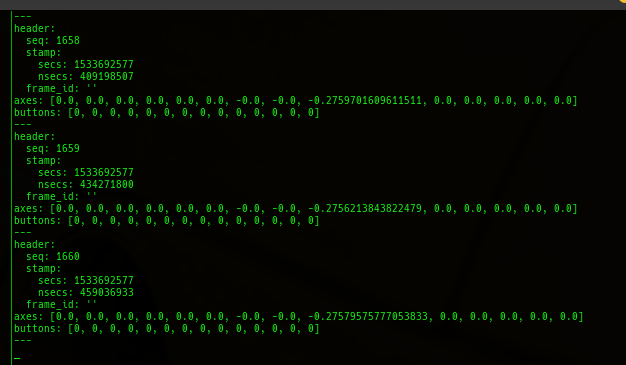
\includegraphics[scale=0.5]{imagenes/joy.png}
\caption{Muestra de la salida del nodo \textit{ps4-ros}. Autoría propia. }
\label{F:joy}
\end{figure}

El producto que genera este módulo, es la publicación de botones y estados de los joystick, en un tópico llamado \textit{\textbackslash joy} (ver figura \ref{F:joy}). Esta información debe ser convertida primero a información compatible para el tópico \textit{\textbackslash cmd\_vel}. El nodo se levanta corriendo el siguiente comando:

\begin{lstlisting}
rosrun ps4-ros ps4-ros
\end{lstlisting}

Un módulo llamado \href{http://wiki.ros.org/teleop_twist_joy}{teleop\_twist\_joy} realiza la función de convertir la información de un mensaje del tipo \textit{\textbackslash joy} a información del tipo \textit{\textbackslash twist}, en un tópico llamado \textit{cmd\_vel}. El nodo se levanta utilizando el siguiente comando:

\begin{lstlisting}
roslaunch teleop_twist_joy bringup.launch
\end{lstlisting}

En la figura \ref{F:omnips4} se muestra la conexión establecida entre el control de PS4 y la computadora principal.

\begin{figure}[H]
\centering
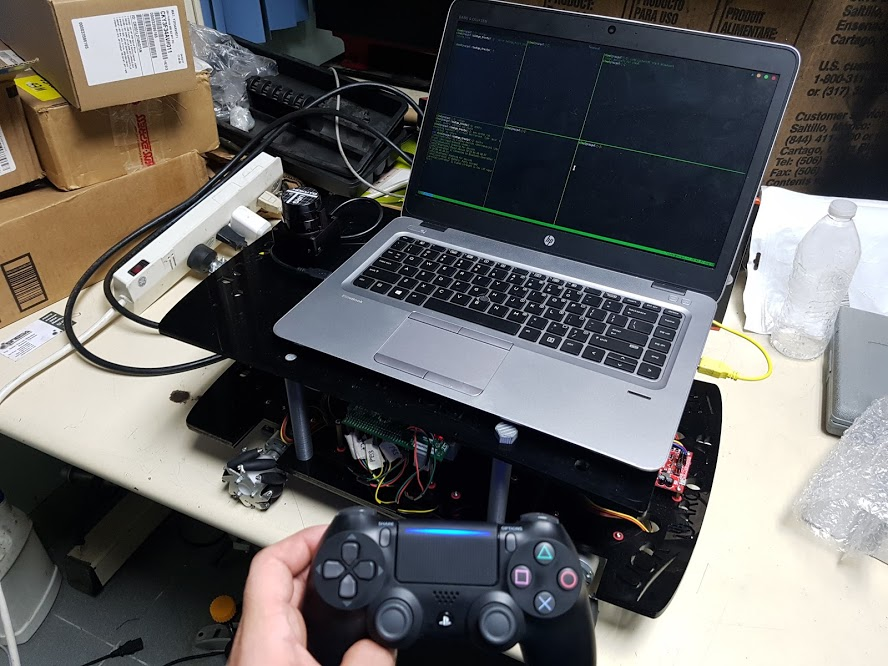
\includegraphics[scale=0.5]{imagenes/ds4omni.jpg}
\caption{Uso del control de PS4 para enviar comandos hacia el robot de velocidad. Autoría propia. }
\label{F:omnips4}
\end{figure}

Algunos videos de muestra se pueden mostrar en el siguiente \href{https://photos.app.goo.gl/rTe4iRubT16syikD7}{link}. Acá se prueba el movimiento lateral, y frontal. Este \href{https://photos.app.goo.gl/8TJrwLLdDjtWyVjg7}{link} muestra el movimiento de la odometría y TF utilizando movimientos en el joystick.

\section{Implementación de Navegación}

Para este punto, se logró implementar correctamente lo siguiente:

\begin{itemize}
\item Se habilita la recepción de comandos de velocidad a través del \
  tópico llamado \textit{cmd\_vel}.
\item Se publica información de la odometría del robot a través del \
  tópico llamado \textit{odom}
\item Se publica la información de los sensores láser en el tópico \
  llamado \textit{laser}
\item Se publica la información de las transformacioens entre el mapa,
  la posición global, la posición de la base del robot, la base del láser,
  y la información de la odometría y la información del láser correspondientemente.
\item Se habilita el nodo llamado \textit{gmapping} para iniciar el
  proceso de mapeo.
\end{itemize}

Para habilitar la navegación en el robot, se creó una guía en el repositorio
en donde están las instrucciones necesarias para realizar el inicio del
mapeo: \href{https://gitlab.com/arcoslab/omnidirectional\_robot/blob/develop/NAVIGATION\_SETUP.md}{NAVIGATION}

Básicamente, una vez que se tiene corriendo el nodo \textit{teleop\_twist\_joy}
se debe correr el nodo \textit{omnidirectional\_node}, el cuál levanta
los procesos de comunicación con la base.

\begin{lstlisting}
  roslaunch omnidirectional_node bringup.launch
\end{lstlisting}

Finalmente, corremos el nodo que controla el láser utilizado para realizar las
pruebas: \textit{hokuyo\_node}. Y por último correr el proceso de mapeo
sobre el tópico \textit{scan}:

\begin{lstlisting}
rosparam set hokuyo_node/port /dev/ttyACM1
rosrun hokuyo_node hokuyo_node
\end{lstlisting}

En los comandos de arriba, se debe verificar cuál es el puerto serial al
cuál se tiene conectado el sensor láser.

Y finalmente, iniciar el proceso de mapeo:

\begin{lstlisting}
  rosrun gmapping slam_gmapping scan:=scan
\end{lstlisting}

Para salvar el mapa que se crea, se debe ejecutar el siguiente comando:

\begin{lstlisting}
rosrun map_server map_saver -f mymap
\end{lstlisting}

\subsection{Configuración}

Se deben definir varios parámetros importantes, los cuáles son:

\begin{itemize}
\item map\_update\_interval: Es el tiempo en segundos entre dos actualizaciones del mapa. Idealmente, la actualización sería instantánea, sin embargo es muy costoso en términos de procesamiento realizarlo de esta manera. El intervalo por defecto es de 5 segundos.

\item max\_Urange: El rango máximo para el cuál el láser brinda información válida. La información que se encuentre más lejos que esta distancia será descartada.

\item iterations: La cantidad de iteraciones del scanmatcher.

\item particles: El número de particulas usadas en el filtro.

\item xmin, ymin, xmax, y ymax: Las coordenadas juntas describen el tamaño del mapa.

\item base\_frame: Indica cuál marco corresponde a la base del robot en el árbol de transformaciones.

\end{itemize}

En lo que respecta al módulo \textit{move\_base}, basa sus técnicas de planeación en la ubicación actual y el destino final. En el código de launch file, se tiene la sintaxis común de un archivo launch, donde se deben definir siete parámetros.

\begin{itemize}

\item base\_global\_planner: Selecciona el plugin a utilizar. Por defecto, se utiliza el de la serie 1.1

\item controller\_frequency: Es un parámetro que fija la frecuencia con la que se mandan comandos de velocidad hacia la base.

\end{itemize}

Además, en el archivo de configuración para el mapa de costos, \textit{costmap\_common\_params} se deben definir ciertos parámetros que usará el \textit{global\_planner}. Por ejemplo:

\begin{itemize}
\item obstacle\_range and raytrace\_range: La distancia mínima en metros que será considerada a la hora de tomar información de un obstáculo y ponerlo en el mapa de costos. Raytrace\_range es la distancia máxima que será considerada cuando se toma espacio libre alrededor de un robot y se agrega en un mapa de costos.

\end{itemize}


\begin{figure}
\centering
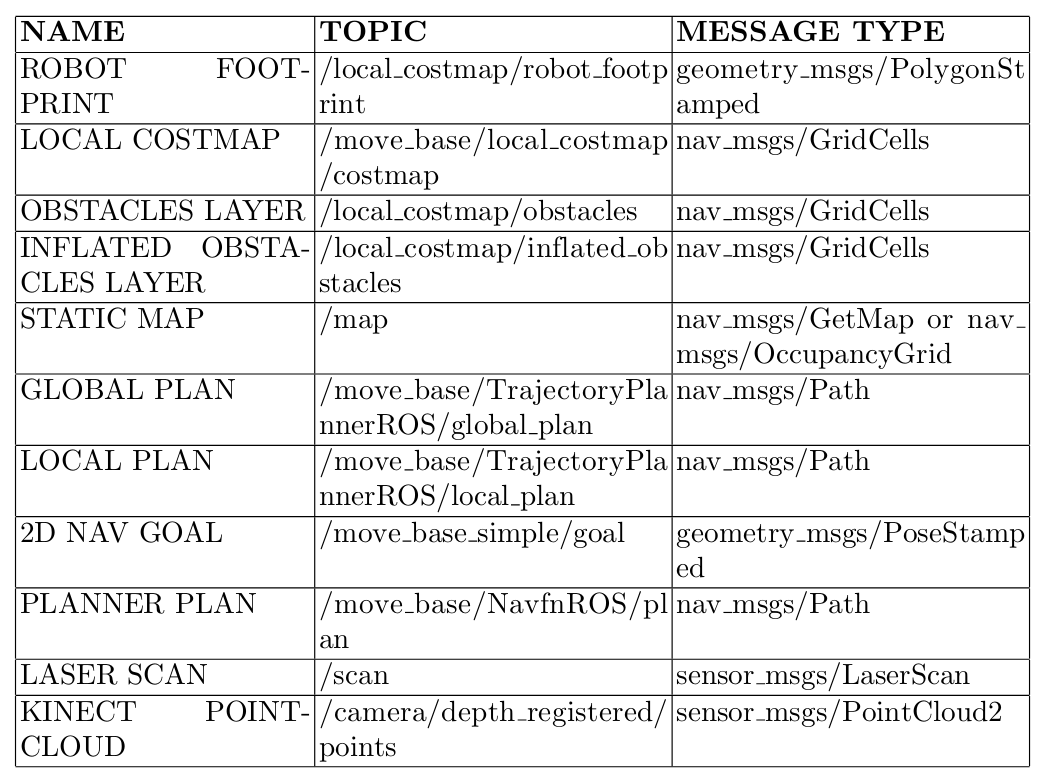
\includegraphics[scale=0.3]{imagenes/tablarequisitos.png}
\caption{Algunos de los requisitos necesarios para la navegación con ROS. Tomado de \cite{Longhi}.}
\label{F:tablanavegacion}
\end{figure}


\subsection{Resultados del mapeo}

Para esta sección, se requirió depurar el código desarrollado del lado del
stm32f4. La odometría de las ruedas tenía un error mayor al 10\% en movientos
lineales y de hasta un 40\% en movimientos traslacionales, lo cuál significa
que el proceso de mapeo no funcionaba correctamente.

Para esta correción, se requirió depurar la manera en la que se calcula la
velocidad del lado del microcontrolador, y además implementar nuevas funciones
en la librería de comunicación serial para determinar cuál era el fallo.

Finalmente, se logró corregir el error, y se iniciaron los primeros mapeos, los
cuáles se muestran a continuacón:

\begin{figure}
\centering
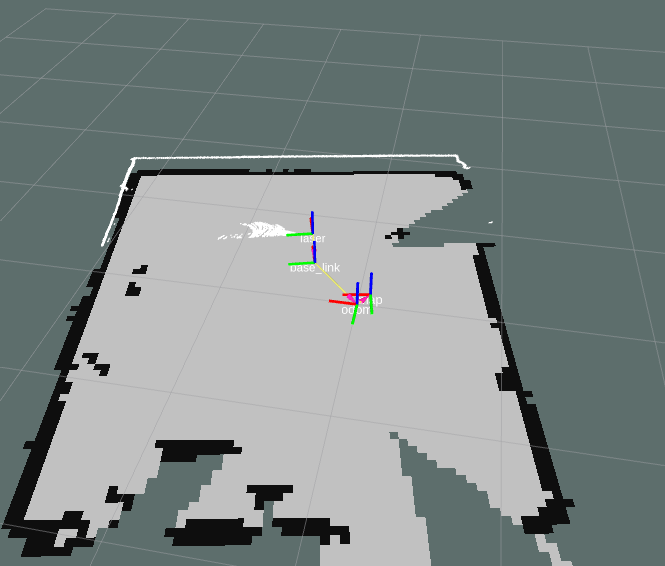
\includegraphics[scale=0.6]{imagenes/mapeo_ini_cocina.png}
\caption{Mapeo realizado en el cuarto de la cocina del INII. Autoría propia.}
\end{figure}

\begin{figure}
\centering
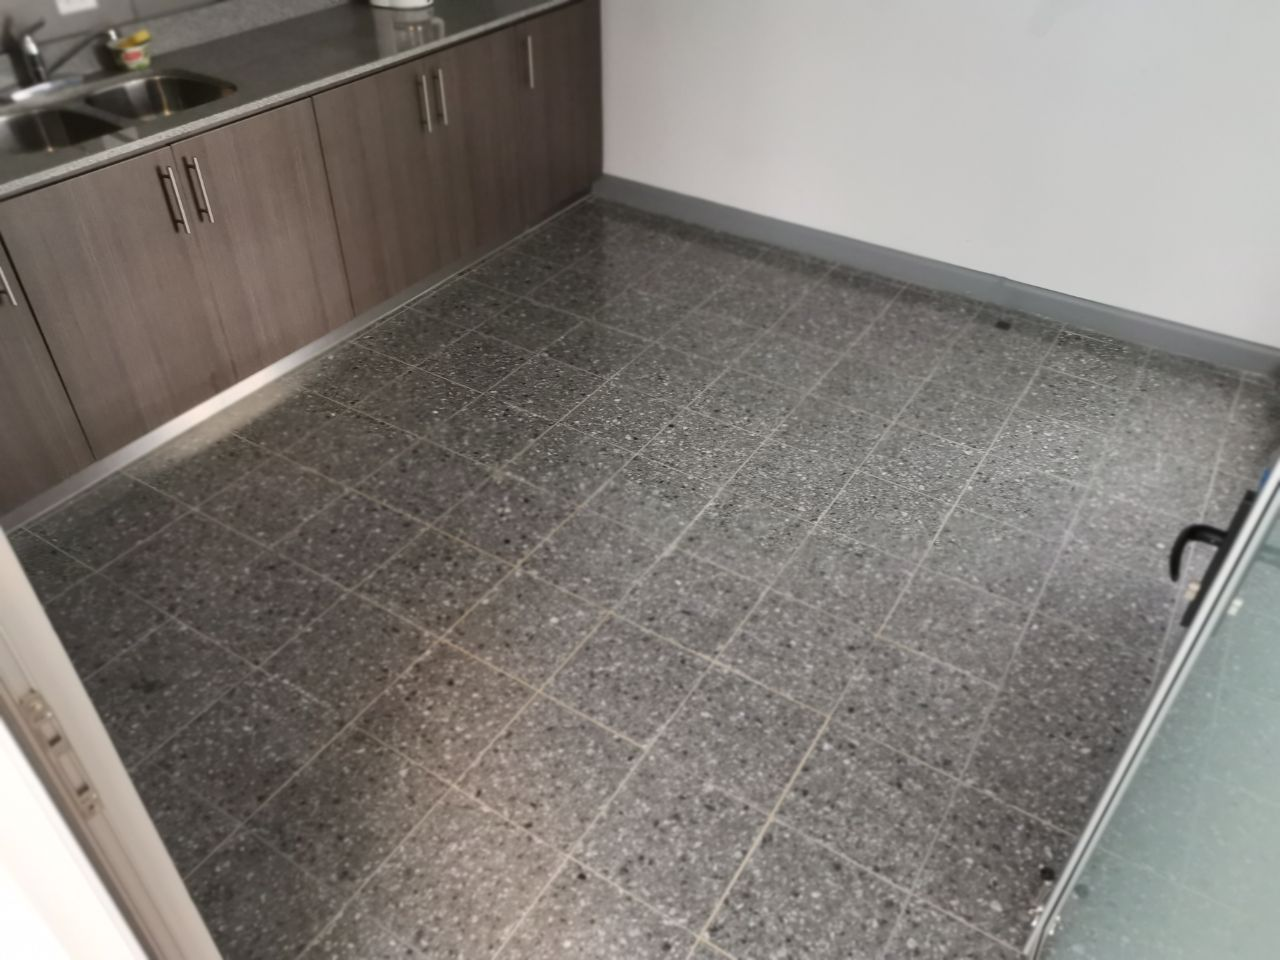
\includegraphics[scale=0.3]{imagenes/cocineta.jpg}
\caption{Fotografía real de la cocineta en la que realizó el mapeo anterior.}
\end{figure}

\begin{figure}
\centering
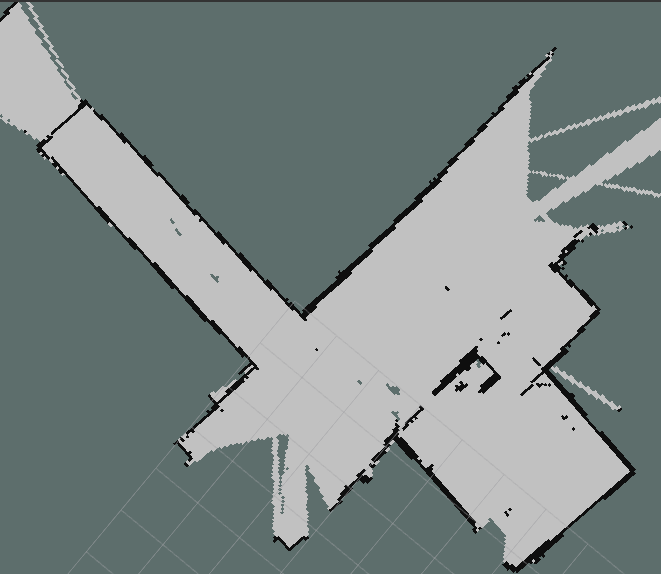
\includegraphics[scale=0.6]{imagenes/mapeo_ini_sur.png}
\caption{Mapeo realizado en el ala Sur del INII. Autoría propia.}
\end{figure}

\begin{figure}
\centering
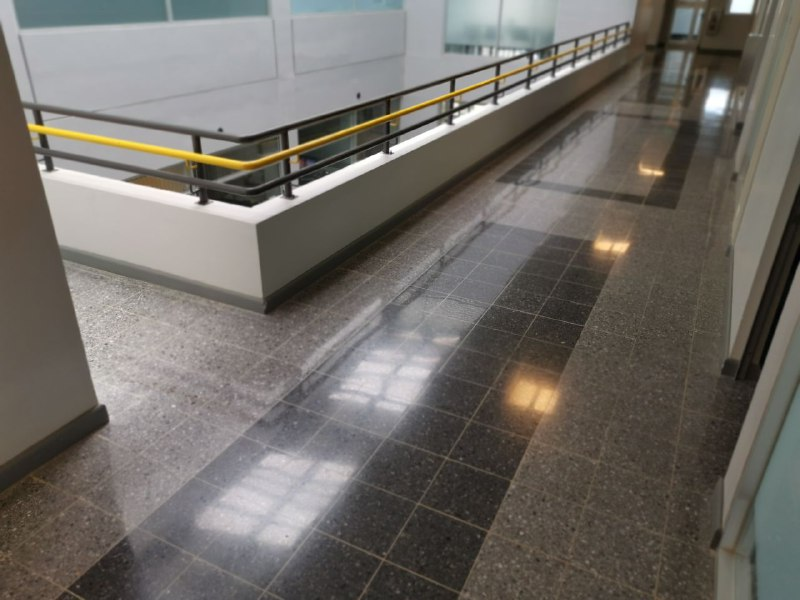
\includegraphics[scale=0.5]{imagenes/pasillo_ini.jpg}
\caption{Fotografía real del pasillo en el que se realizó el mapeo anterior.}
\end{figure}

\begin{figure}
\centering
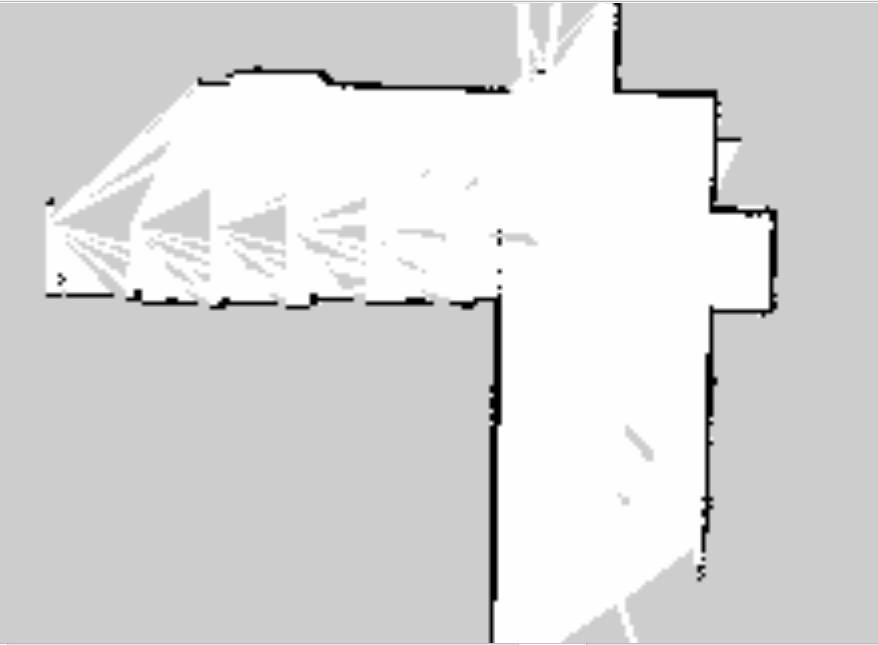
\includegraphics[scale=0.5]{imagenes/mapeo_esquina.png}
\caption{Mapeo realizado en la esquina a las afueras del ARCOS-LAB. Autoría propia.}
\end{figure}

\begin{figure}
\centering
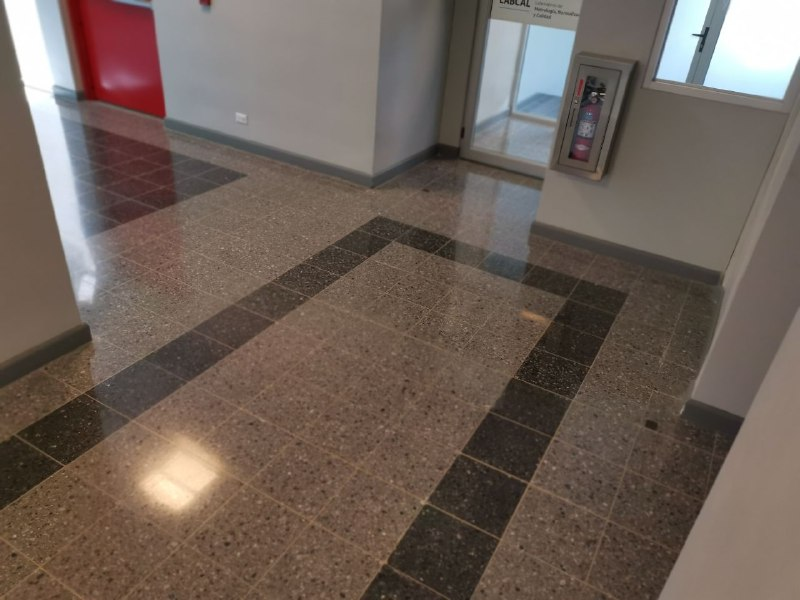
\includegraphics[scale=0.5]{imagenes/afueras_arcoslab.jpg}
\caption{Fotografía real del pasillo en el que se realizó el mapeo anterior.}
\end{figure}

\subsection{Problemas}

Como se mencionó anteriormente, para esta sección se debieron corregir algunos
problemas encontrados durante la implementación de los cálculos de la
odometría del robot.

Sin embargo, propiamente con esta sección no se encontraron errores importantes.

El único error que cabe rescatar, es que inicialmente se inició con una
transformación del láser, en la dirección relativa a la base incorrecta.
Esto causaba que virtualmente, el láser estuviera atrás del centro del robot,
pero en la realidad estaba delante del robot.

Este error pudo ser detectado por el profesor Federico Ruíz, al sugerir
realizar movimientos circulares en los cuáles se evidencia más este error.

